\documentclass[../main.tex]{subfiles}
\begin{document}


\chapter{La huerta agroecológica y sus fundamentos}

Una \tcbox{huerta} nos permite obtener alimentos naturales, independientes, de un origen conocido y sobre el que tenemos control; el usar un \tcbox{método agroecológico} de cultivo nos facilita la tarea de cosechar hortalizas saludables, libres de agrotóxicos y sin el riesgo al que nos exponemos como consecuencia de los productos utilizados en la producción industrial de alimentos. 



\section{¿Qué es una huerta agroecológica?}

El cultivo agroecológico es un conjunto de prácticas que busca producir alimentos de manera estable y efectiva aprovechando los recursos propios de la naturaleza minimizando el daño que les producimos. 

La agroecología es una combinación entre aspectos científicos y sociales que se apoya fuertemente en la sostenibilidad, llevando a favorecer ciertas maneras de relacionarse con el ambiente, que promueven la salud humana y ambiental, el respeto y cuidado del medio ambiente, y que buscan mejorar la calidad y cantidad de elementos que podemos aprovechar de la naturaleza.\\

\begin{recuadroV}
    Por lo tanto el objetivo de una huerta agroecológica no reside únicamente en la neta producción de alimentos, si no en el empoderamiento de quienes participan en su construcción y el control sobre lo que consumimos, manteniendo la economía, el respeto y sostenibilidad necesarios para coexistir con la naturaleza.
\end{recuadroV}


\hfill\\

Ciertas condiciones deben cumplirse para que podamos acercarnos a ese objetivo:\\

\begin{itemize}
    \item Nunca se usan productos “agrotóxicos” porque alteran el medio ambiente y pueden dañar directamente nuestra salud.
    \item Se mejora y fertiliza el suelo con \tcbox{abonos naturales} u orgánicos.
    \item Se siembra una gran variedad de hortalizas y hierbas para mantener el equilibrio biológico en la huerta.
    \item \color{black!50}{Se asocian los cultivos para no exigir a la tierra\\ los mismos nutrientes.} \observation{¿Qué significa esto?}
    \item \color{black}Se desarrolla la rotación adecuada para obtener plantas vigorosas y para no agotar a la tierra.
\end{itemize}

\hfill\\

\begin{wrapfigure}[13]{o}[0cm]{0.45\textwidth}
    \centering
    \begin{tikzpicture}
        \def\ig{%
         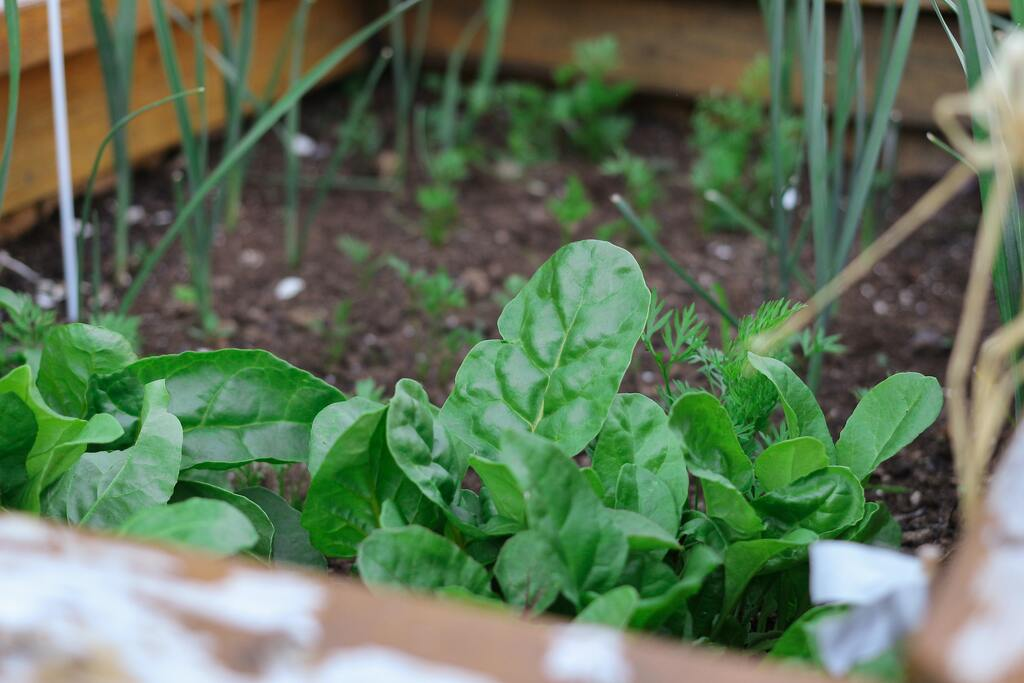
\includegraphics[width={0.4\textwidth},keepaspectratio]{huerta/1b.jpg}}
       \node [inner sep=0pt](image) at (0,0) {\phantom{\ig}};
       \clip[rounded corners=5mm] ($(image.south west)+(\bord,\bord)$) rectangle ($(image.north east)-(\bord,\bord)$);
       \node[inner sep=0pt](image) at (0,0) {\ig};
      \end{tikzpicture}
    \caption*{\color{CompostGreen!50!black}Las hortalizas en nuestra huerta}
    \label{hortalizas1}
\end{wrapfigure}


Cultivar hortalizas agroecológicas nos permite tener una variedad de alimentos sanos, frescos, nutritivos y sabrosos, libres de sustancias tóxicas a un costo bajo, además de colaborar con un espacio verde y participativo en el hogar o en la comunidad. \\

Las hortalizas y verduras son alimentos indispensables en nuestra alimentación, aportan fibras, agua, antioxidantes y vitaminas, tienen  un papel trascendental en el equilibrio de nuestra dieta.\\


Generalmente se las clasifica según su parte comestible: 
\hfill\\
\begin{itemize}
    \item \textbf{Raíz}: zanahoria, nabo, remolacha, rabanito.
    \item \textbf{Hoja}: apio, perejil, acelga, espinaca, lechuga, cebolla de hoja.
    \item \textbf{Tallos y bulbos}: cebolla, ajo, papa.
    \item \textbf{Flor}: coliflor, brócoli.
    \item \textbf{Fruto}: tomate, pepino, zapallo, haba, arveja, ají, pimiento, berenjena.
\end{itemize}

\hfill\\

Es importante entender las diferencias y características particulares entre las diversas hortalizas y qué nos conviene plantar en función de nuestras necesidades particulares, por lo que este tipo de clasificaciones es útil para facilitar la discriminación de los alimentos que vamos a poner en nuestra huerta.


\section{Consideraciones previas a su creación}

Así como hay lineamientos que cumplir con respecto a la siembra y la cosecha, hay pasos que debemos tener en cuenta antes de decidir cómo y dónde hacer nuestra huerta.

\hfill\\

\begin{recuadroR}
    Es importante tomarse el tiempo de determinar correctamente estos pasos antes de comenzar a trabajar la tierra, ya que darse cuenta que algo no va a funcionar bien una vez que está sembrado significaría destruir toda la huerta.
\end{recuadroR}

\hfill\\

El terreno para hacer nuestra huerta debe estar \tcbox{cerca de una fuente de agua}; un grifo, pozo o un rio, y no debe estar muy alejado del hogar o de la escuela para facilitar su trabajo y su cuidado. 

Debemos considerar la inclinación del terreno, el tipo y condiciones del suelo que tenemos (arena o arcilla, presencia de piedras). El terreno no debe tener piedras en profundidad ya que será difícil quitarlas y además evitarán que las raíces de las plantas se desarrollen adecuadamente. \\

Es conveniente que la huerta tenga \tcbox{acceso a la luz solar} (recomendable de 6 a 8 horas/día). Debe  estar alejada de paredones o de árboles que hagan demasiada sombra. Es recomendable que haya árboles o cercos vivos alrededor para protegerla de vientos y temperaturas extremas.

El terreno debe contener \tcbox{suelo limpio}, donde no haya presencia de basura o elementos que puedan contaminar la huerta, como ser latas, plásticos o colillas de cigarrillos. \\

Hay que tener en cuenta que si el área a sembrar es suficientemente grande hay que agregar espacios o corredores, para que las personas puedan transitar, hacer mantenimiento, sembrar y realizar la cosecha.


\section{Su construcción}

Una vez tenemos determinado dónde estará ubicada la huerta, y su configuración, podemos comenzar con el proceso inicial de construcción de la huerta en sí misma.

\subsection{Preparación del terreno}

Antes de sembrar en la huerta debemos preparar el terreno.\\


Se recomienda \tcbox{cercar la huerta} para que no entre ningún animal, ya que pueden destruir la siembra, ya sea comiéndosela, cavando o por el mero hecho de haber entrado y pisado donde no debían. 
La cerca se puede construir de forma económica con postes o estacas de madera y alambre o mallado que permita que circule aire, insectos y partículas, pero debemos evitar el paso de cualquier animal grande. Otra alternativa son las cercas vivas, que se pueden hacer de plantas fuertes o espinosas, teniendo en cuenta que hay que también hay que mantener las plantas de cerco y que pueden tomar un tiempo antes de tener un tamaño o ser suficientemente frondosas para que sean efectivas como barrera. \\

\begin{wrapfigure}[20]{o}[0cm]{0.45\textwidth}
    \centering
    \begin{tikzpicture}
        \def\ig{%
         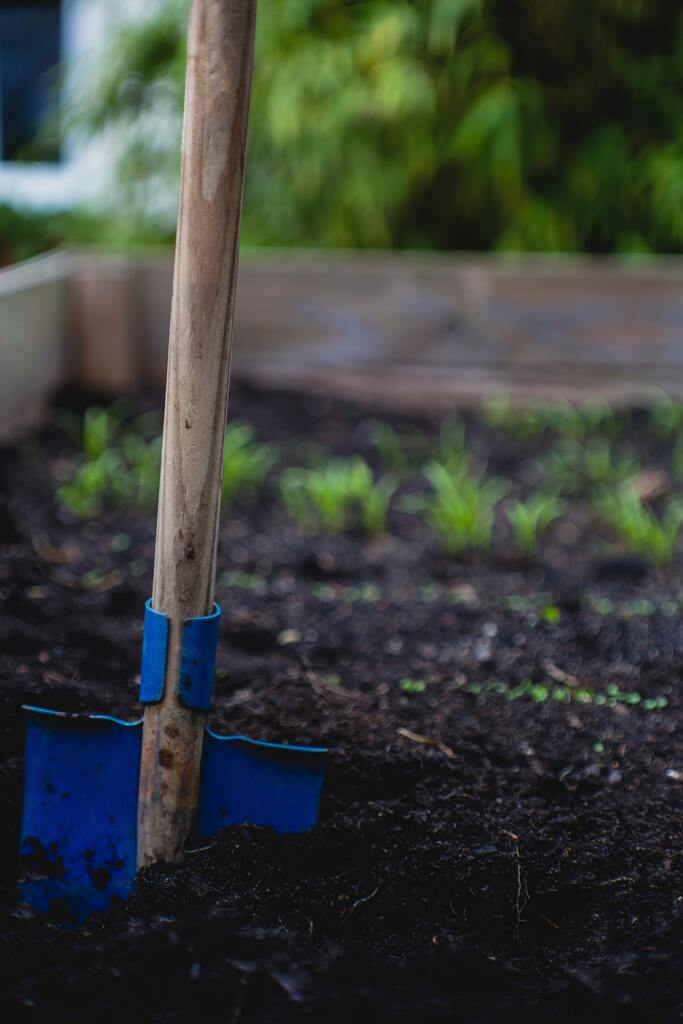
\includegraphics[width={0.4\textwidth},keepaspectratio]{huerta/5.jpg}}
       \node [inner sep=0pt](image) at (0,0) {\phantom{\ig}};
       \clip[rounded corners=5mm] ($(image.south west)+(\bord,\bord)$) rectangle ($(image.north east)-(\bord,\bord)$);
       \node[inner sep=0pt](image) at (0,0) {\ig};
      \end{tikzpicture}
    \caption*{\color{CompostGreen!50!black}La preparación del terreno}
    \label{prep1}
\end{wrapfigure}

Se debe \tcbox{limpiar el terreno} de piedras, palos, raíces y hierbas que preferimos evitar que estén ahí. También podemos humedecer el suelo para que sea menos trabajoso limpiarlo, ya que es una tarea pesada que involucra mucho trabajo manual ya sea con herramientas, como una azada, o directamente con la mano. \\
Con un suelo limpio podemos preparar la tierra aflojándola, deshaciendo los terrones y asegurándonos de que quede suficientemente suelta y acolchonada para que las semillas puedan acomodarse felices. \\

Una vez removida la tierra tenemos que \tcbox{abonarla} con nutrientes: materia orgánica que enriquezca la calidad del suelo y mejore su composición. 

\hfill\\

\begin{recuadroV}
    Recordemos que el suelo donde vamos a sembrar no está compuesto meramente por tierra existiendo en un vacío, es una composición compleja de diversos nutrientes, elementos orgánicos e inorgánicos y fauna microscópica, por lo que es importante hacer lo equivalente a darle de comer y alterar las proporciones de nutrientes y materia orgánica presente para que sea más amigable para las plantas.
\end{recuadroV}

\hfill\\

Para esto podemos utilizar mantillo o \tcbox{abono orgánico} (compost o lombricompost), que es efectivo, se puede producir como resultado de nuestro consumo personal de alimentos, y no altera de forma adversa el ambiente ni induce compuestos que o desconocemos el efecto que pueden tener sobre los consumidores, o sabemos que pueden ser nocivos. También tiene la ventaja de que en general evitará el crecimiento natural de las hierbas que queremos evitar tener en la huerta. \\

\subsection{Los tablones}


Con el terreno listo se puede pasar a la preparación de \tcbox{los tablones}; se le suele llamar tablón al emplazamiento de terreno donde directamente se realizará la siembra. Los tablones se pueden marcar con estacas e hilos, y cada uno debe tener entre 1 y 1.2 metros de ancho, y un largo entre 5 y 6 metros, aunque podemos llegar a estirarnos hasta 10 metros. \\
Para caminar sin problemas por la huerta conviene espaciar los tablones por aproximadamente medio metro. 



\begin{wrapfigure}[13]{o}[0cm]{0.45\textwidth}
    \centering
    \begin{tikzpicture}
        \def\ig{%
         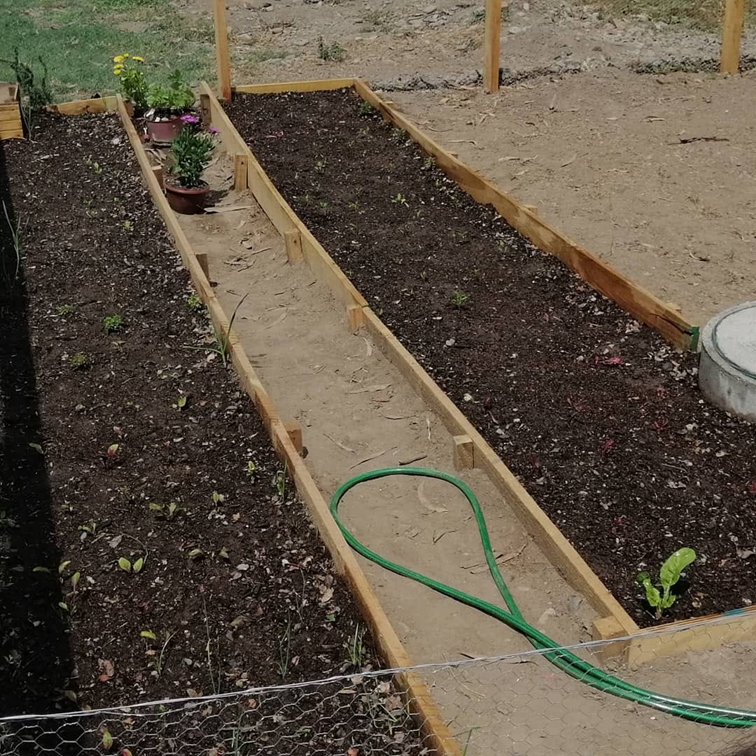
\includegraphics[width={0.4\textwidth},keepaspectratio]{huerta/2.png}}
       \node [inner sep=0pt](image) at (0,0) {\phantom{\ig}};
       \clip[rounded corners=5mm] ($(image.south west)+(\bord,\bord)$) rectangle ($(image.north east)-(\bord,\bord)$);
       \node[inner sep=0pt](image) at (0,0) {\ig};
      \end{tikzpicture}
    \caption*{\color{CompostGreen!50!black}Los tablones en nuestra huerta}
    \label{tablones1}
\end{wrapfigure}

\section{La siembra}

Teniendo el suelo listo, el siguiente paso es la siembra. \\ 

Existen principalmente dos tipos: la \emph{directa} y la siembra \emph{en almácigos}.

La siembra directa consiste en, según el caso, disponer de las semillas de manera directa sobre la tierra. Por su parte, algunas hortalizas necesitan un mayor cuidado inicial, por lo que plantamos sobre segmentos de tierra aislados e independientes que llamamos almácigos.
 
\subsection{Siembra directa}

Utilizaremos la siembra directa para las semillas grandes, fáciles de manejar y fuertes para germinar (zapallo, zapallito, melón, maíz, poroto, sandía). También requieren de este tipo de siembra aquellas especies que no toleran el trasplante (zanahoria, perejil, rabanito, achicoria, espinaca, remolacha).\\

\hfill\\

La siembra directa tiene varios subtipos:

\hfill\\

\begin{itemize}
    \item \textbf{A golpe}: se siembran grupos de 3 a 5 semillas, ya que algunas pueden no germinar. La distancia de siembra depende de cada especie (zapallos, sandias, melones).
    \item \textbf{En línea o a chorillo}: se marcan líneas o surcos donde se sembrarán (semillas pequeñas como ser la rúcula) .
    \item \textbf{Al voleo}: consiste en esparcir las semillas de manera uniforme en una superficie (no es conveniente).
\end{itemize}

\hfill\\

La distancia entre la siembra dependerá de la planta y el espacio que necesite para desarrollarse, puede consultarse en el \appendixbox{\hyperref[appendixA]{Apéndice \ref{appendixA}}}. La profundidad de siembra es tres veces el tamaño de la semilla. Podemos cubrir las semillas con más compost y presionamos apenas. Luego regamos con una lluvia fina.

\hfill\\

\begin{recuadroV}
    Recordemos: la siembra directa se realiza para especies que no toleran transplantes, y las semillas grandes, fuertes y fáciles de manejar.
\end{recuadroV}
 
\subsection{Siembra en almácigos}

Algunas hortalizas tienen semillas pequeñas y son más delicadas. Por eso, las sembramos en un espacio pequeño que llamamos almácigo. \\

Para preparar los almácigos, podemos utilizar cajas de madera (de verdulería), latas, envases de poliestireno expandido (conocido como telgopor) o plástico, hueveras de cartón corrugado, macetas, o cualquier envase similar que \tcbox{no sea tóxico} para la tierra o las plantas. \\

Es importante realizar cortes en el fondo del envase para permitir el drenaje. Dentro del envase que hayamos elegido debemos colocar la tierra enriquecida con compost (tierra fértil). Esta tierra debe ser tan fina como sea posible. Colocamos las semillas de acuerdo a tamaño del recipiente de almácigo y lo regamos. El \tcbox{riego debe ser cuidadoso}, a modo de goteo o de lluvia. Los almácigos deben estar en un lugar que no estén expuestos a corrientes de aire, ni al sol directo. \\


\begin{wrapfigure}[12]{o}[0cm]{0.45\textwidth}
    \centering
    \begin{tikzpicture}
        \def\ig{%
         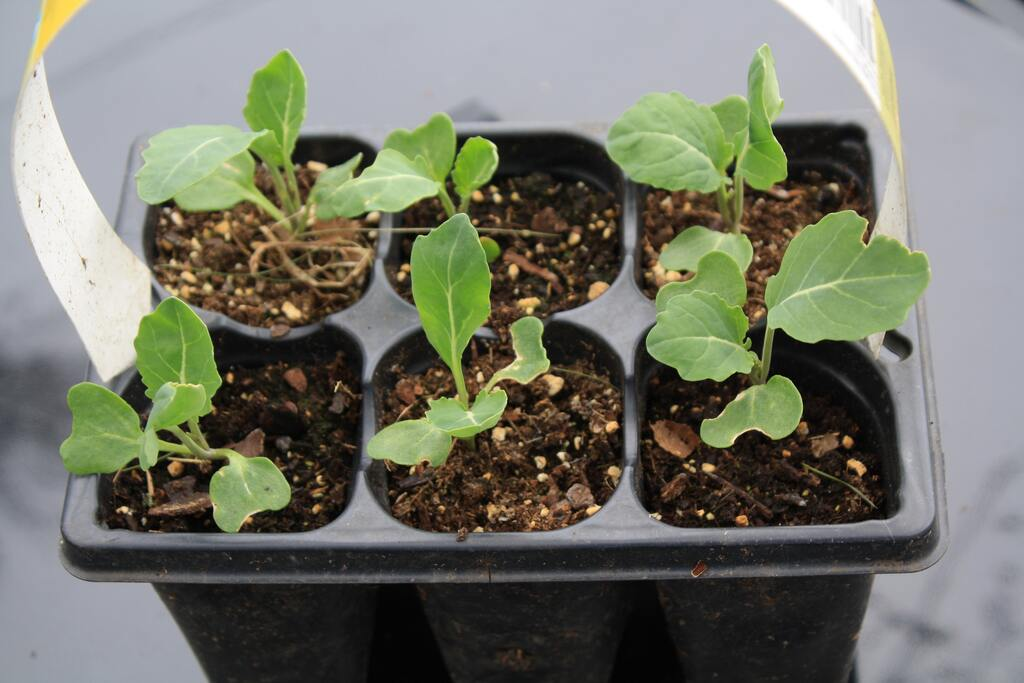
\includegraphics[width={0.4\textwidth},keepaspectratio]{huerta/3.jpg}}
       \node [inner sep=0pt](image) at (0,0) {\phantom{\ig}};
       \clip[rounded corners=5mm] ($(image.south west)+(\bord,\bord)$) rectangle ($(image.north east)-(\bord,\bord)$);
       \node[inner sep=0pt](image) at (0,0) {\ig};
      \end{tikzpicture}
    \caption*{\color{CompostGreen!50!black}Los almácigos}
    \label{almacigo1}
\end{wrapfigure}

Cuando las plantas tengan 3 o 4 hojas (lechuga, repollo, acelga, coliflor) o cuando el tallo llega al grosor de un lápiz (tomate, berenjena, puerros, pimientos), los plantines están listos para ser trasplantados.\\
El trasplante debe hacerse con sumo cuidado para no lastimar las raíces. Puede hacerse moviendo el plantín con toda la tierra que había en el almácigo (si se hace en vasitos) o (si, por ejemplo, se elige hacerlo en un cajón de madera) abriendo un agujero alrededor de la planta con un cuchillo de cocina o con una lapicera en desuso y levantando el plantín con la mano. En el traslado, debemos evitar que se desprenda la tierra de las raíces. \\


\begin{wrapfigure}[12]{i}[0cm]{0.45\textwidth}
    \centering
    \begin{tikzpicture}
        \def\ig{%
         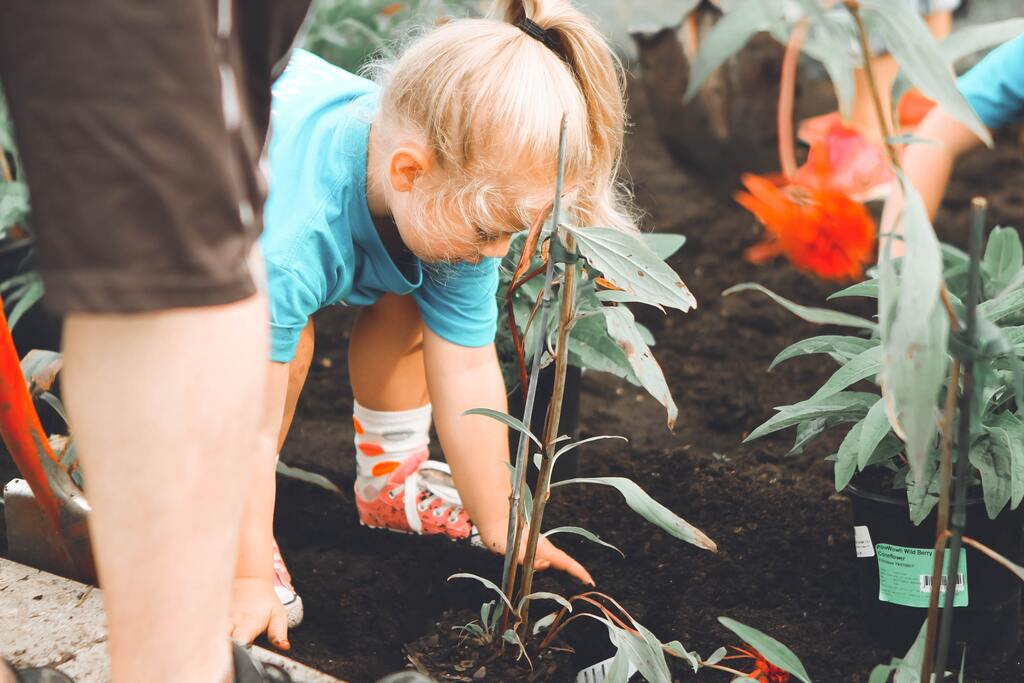
\includegraphics[width={0.4\textwidth},keepaspectratio]{huerta/4.jpg}}
       \node [inner sep=0pt](image) at (0,0) {\phantom{\ig}};
       \clip[rounded corners=5mm] ($(image.south west)+(\bord,\bord)$) rectangle ($(image.north east)-(\bord,\bord)$);
       \node[inner sep=0pt](image) at (0,0) {\ig};
      \end{tikzpicture}
    \caption*{\color{CompostGreen!50!black}El transplante}
    \label{transplante1}
\end{wrapfigure}


En el lugar en el que van a ubicarse los plantines se preparan pequeños hoyos, con una profundidad necesaria para que se pueda colocar el plantín y su raíz. La distancia entre los plantines dependerá de la planta y el espacio que necesite para desarrollarse, puede consultarse en el \appendixbox{\hyperref[appendixA]{Apéndice \ref{appendixA}}}.
Una vez hecho el pase, se termina de tapar con abono compuesto o tierra enriquecida con compost orgánico. Con ambas manos se presiona la tierra junto a la planta, para que quede firme, y se riega alrededor de las plantitas.

\hfill\\

\begin{recuadroV}
    Recordemos: la siembra en almácigos se utiliza para especies delicadas y semillas muy pequeñas. Podemos reciclar envases desechables para crear los almácigos, siempre teniendo cuidado de que no contengan tóxicos que puedan afectar a la tierra o a las plantas, que podemos evitar generalmente lavándolos bien y evitando el uso de contenedores que tuvieron químicos, aceites, solventes, pinturas o demás compuestos agresivos.
\end{recuadroV}

\subsection{Cuidados}

Nuestra huerta ya sembrada requiere de un \tcbox{mantenimiento continuo}, de lo contrario las plantas mueren y no podemos cosechar ningún alimento. Estos cuidados incluyen el regar las plantas, administrar y controlar su crecimiento, mantener el acondicionamiento del terreno y usar aditivos naturales como los que podemos encontrar en el \appendixbox{\hyperref[appendixC]{Apéndice \ref{appendixC}}}.



\subsubsection{Riego}

\begin{wrapfigure}[20]{o}[0cm]{0.45\textwidth}
    \centering
    \begin{tikzpicture}
        \def\ig{%
         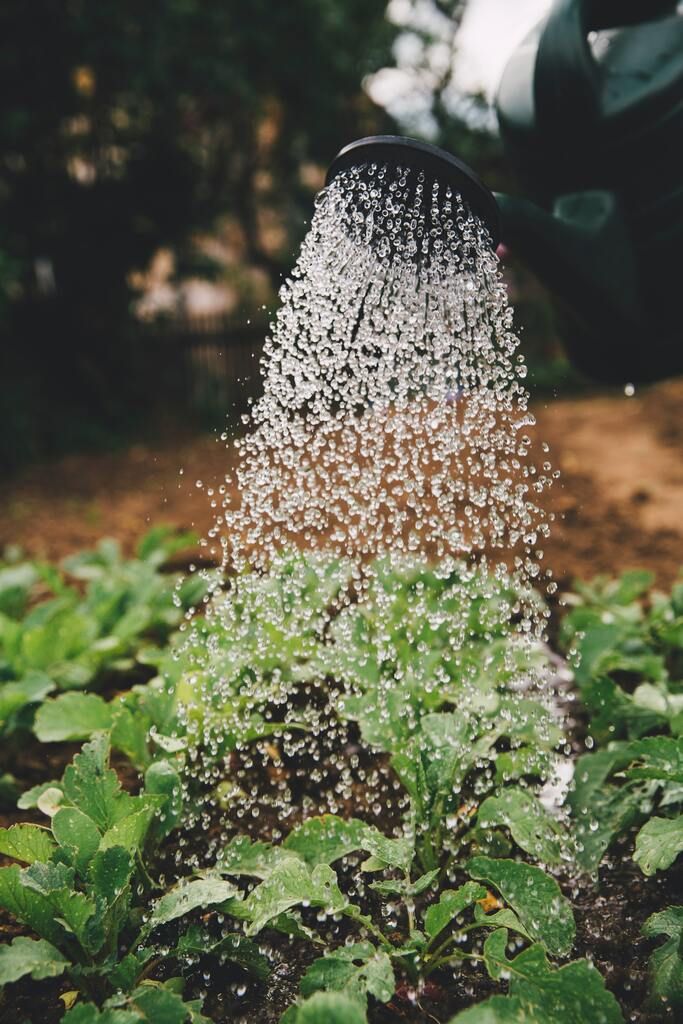
\includegraphics[width={0.4\textwidth},keepaspectratio]{huerta/8.jpg}}
       \node [inner sep=0pt](image) at (0,0) {\phantom{\ig}};
       \clip[rounded corners=5mm] ($(image.south west)+(\bord,\bord)$) rectangle ($(image.north east)-(\bord,\bord)$);
       \node[inner sep=0pt](image) at (0,0) {\ig};
      \end{tikzpicture}
    \caption*{\color{CompostGreen!50!black}Riego}
    \label{riego1}
\end{wrapfigure}

Para el desarrollo de nuestras plantas \tcbox{es imprescindible el riego}. El riego debe ser controlado. Si el agua no es suficiente las plantas no se desarrollan normalmente, y la producción es menor; las hojas se ponen duras y puede ocurrir que las plantas semillen antes de tiempo. Pero también hay que tener cuidado con el exceso de humedad, ya que puede favorecer la aparición de enfermedades y los productos obtenidos serán de mala calidad, menos nutritivos. En el \appendixbox{\hyperref[appendixB]{Apéndice \ref{appendixB}}} podemos ver cómo construir un sistema de riego simple y efectivo.


\subsubsection{Desyerbar o carpir}

Carpir es \tcbox{quitar las hierbas indeseables} para nuestra huerta, que nacen junto al cultivo. Se busca quitarlas porque pueden verse perjudiciales para el sembradío. \\

Se debe realizar periódicamente para evitar la competencia entre malezas y hortalizas por luz, agua, nutrientes y espacio, y especialmente cuando las hortalizas todavía son pequeñas el deshierbe constante tiene una importancia mayor. También hay que tener en cuenta que deben ser removidas antes de tener semillas, y hay que tener cuidado de sacar también la raíz, de manera que no crezcan nuevamente ni se reproduzcan.

\subsubsection{Raleo}

Cuando las plantitas empiezan a crecer y quedan demasiado amontonadas se deben sacar las plantas menos desarrolladas hasta que exista suficiente espacio entre una y otra. El raleo debe ser aplicado lo más temprano posible para que beneficie el crecimiento de las plantas.

\subsubsection{Aflojar la tierra}

Para que las plantas puedan respirar, el agua pueda filtrarse y el terreno no se encharque se debe aflojar la tierra regularmente.


\subsubsection{\hfill{Aporque}}


\begin{wrapfigure}[19]{o}[0cm]{0.45\textwidth}
    \centering
    \begin{tikzpicture}
        \def\ig{%
         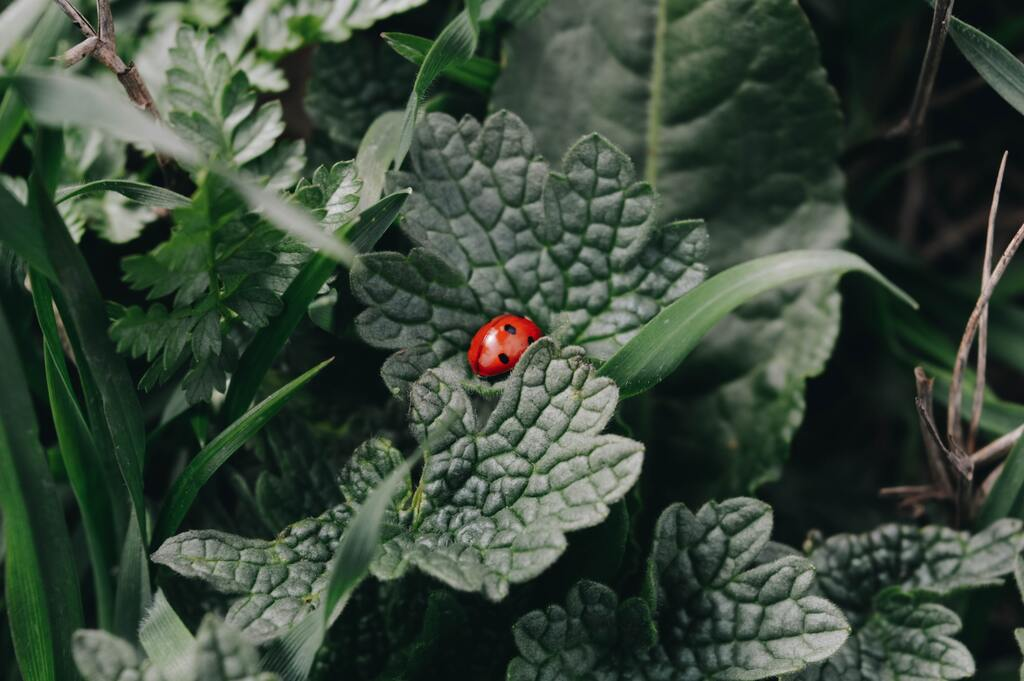
\includegraphics[width={0.4\textwidth},keepaspectratio]{huerta/7.jpg}}
       \node [inner sep=0pt](image) at (0,0) {\phantom{\ig}};
       \clip[rounded corners=5mm] ($(image.south west)+(\bord,\bord)$) rectangle ($(image.north east)-(\bord,\bord)$);
       \node[inner sep=0pt](image) at (0,0) {\ig};
      \end{tikzpicture}
    \caption*{\color{CompostGreen!50!black}El desmalezado}
    \label{desyerbar1}
\end{wrapfigure}

El aporque consiste en acumular tierra en la base del tronco o tallo de una planta con el fin de que quede protegida, para que no reciba directamente el sol, impidiendo también el exceso de humedad.


\subsubsection{Tutoraje}

Algunas hortalizas como el tomate, arveja, o pepino, tienen tallos y ramas frágiles que pueden quebrarse o caerse por el peso de sus frutos. Para ello se amarran las plantas a estacas, caballetes o hilos de alambre, a esto se le llama \emph{tutoraje}.

\subsection{\raggedleft{La cosecha}}

La cosecha es la recompensa por todo el esfuerzo empleado anteriormente en la huerta. Esta actividad se realiza, dependiendo de la planta, \tcbox{entre 90 y 120 días} (tres y cuatro meses) luego de la siembra o trasplante. Para esta actividad, se recomienda utilizar tijeras o cuchillos limpios; además, es recomendable cosechar en el momento que vayamos a consumir los alimentos, de manera que los consumamos frescos y con todos sus nutrientes activos.\\

\begin{wrapfigure}[10]{i}[0cm]{0.45\textwidth}
    \centering
    \begin{tikzpicture}
        \def\ig{%
         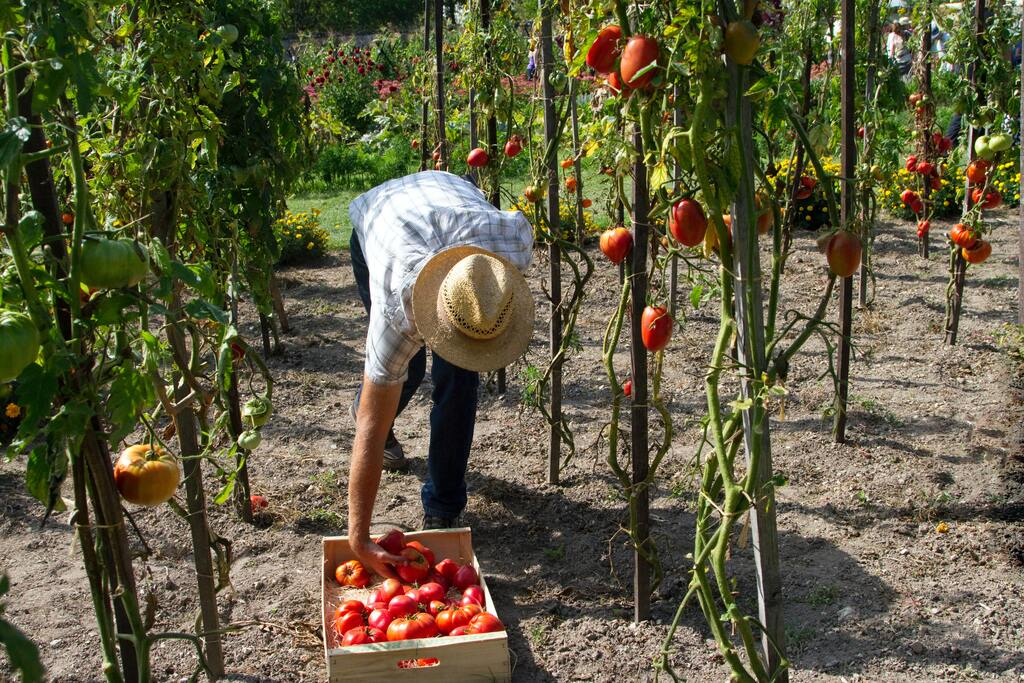
\includegraphics[width={0.4\textwidth},keepaspectratio]{huerta/6.jpg}}
       \node [inner sep=0pt](image) at (0,0) {\phantom{\ig}};
       \clip[rounded corners=5mm] ($(image.south west)+(\bord,\bord)$) rectangle ($(image.north east)-(\bord,\bord)$);
       \node[inner sep=0pt](image) at (0,0) {\ig};
      \end{tikzpicture}
    \caption*{\color{CompostGreen!50!black}El tutoraje}
    \label{tutoraje1}
\end{wrapfigure}

Siempre es bueno saber cuándo cosechar para no dañar nuestras plantas y para tener alimento fresco durante más tiempo. Por ejemplo; la cebolla y el ajo podemos cosecharlos cuando estén tiernos o cuando sus hojas se hayan secado por completo, debido a que el bulbo se conserva muy bien hasta cierto tiempo en el suelo, igualmente con la lechuga, espinaca o acelga. Podemos ir cosechándolas poco a poco, hoja por hoja, dependiendo de la cantidad que necesitemos para la preparación de los alimentos.

\begin{recuadroR}
    El mantenimiento de la huerta puede ser trabajoso, pero es esencial para alcanzar el éxito y obtener alimentos sanos y de calidad. Para limitar un poco esta dificultad, si tenemos la oportunidad, conviene repartir el trabajo entre muchas personas que se responsabilicen de manera alternativa para hacer los cuidados. Esto permitirá que la huerta reciba todo el amor que necesita sin que las personas que la mantienen se cansen.
\end{recuadroR}

\vfill

\begin{figure}[H]
    \centering
    \begin{tikzpicture}
        \def\ig{%
         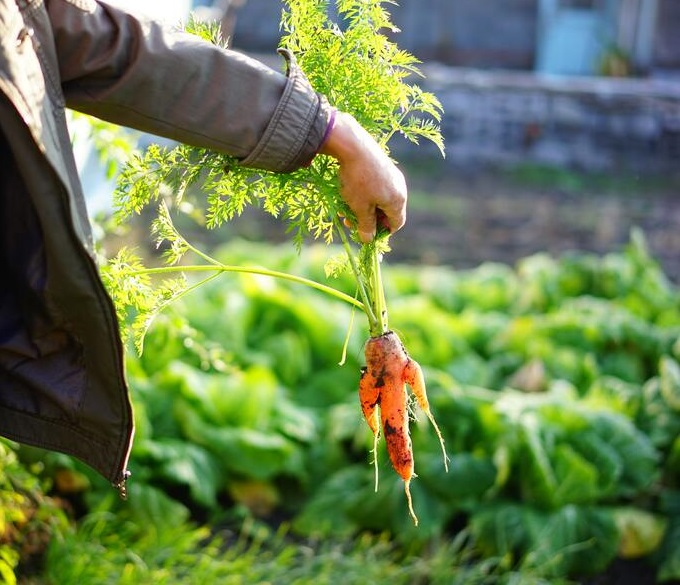
\includegraphics[width={\textwidth},keepaspectratio]{huerta/9.jpg}}
       \node [inner sep=0pt](image) at (0,0) {\phantom{\ig}};
       \clip[rounded corners=5mm] ($(image.south west)+(\bord,\bord)$) rectangle ($(image.north east)-(\bord,\bord)$);
       \node[inner sep=0pt](image) at (0,0) {\ig};
      \end{tikzpicture}
    \caption*{\color{CompostGreen!50!black}La cosecha: el resultado de nuestros esfuerzos}
    \label{cosecha1}
\end{figure}


\vfill

\pagebreak



\end{document}